\documentclass[../main]{subfiles}
\begin{document}

\Large
\begin{tabu}{clr}
  \multirow{6}{1in}{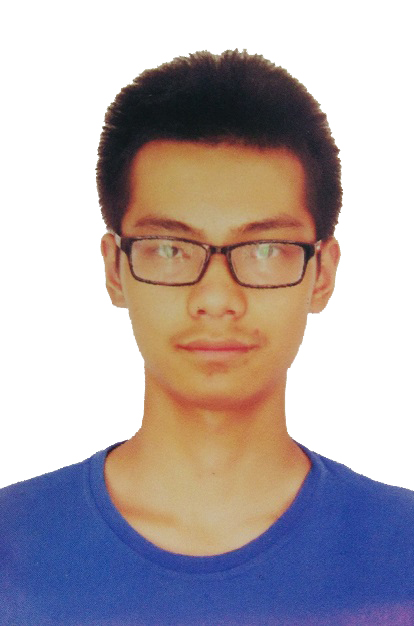
\includegraphics[width=0.88in]{images/profile.jpg}} & \faMale\
  \scshape{吴振宇}                                                         & {\faPython\ Python~}\progressbar{0.95}                                                    \\
                                                                        & \email{wuzhenyu@ustc.edu}                          & {\faDraftingCompass\
  Perl~}\progressbar{0.8}                                                                                                                                           \\
                                                                        & \phone{+86~183~555~28308}                          & {\faLinux\ Linux~}\progressbar{0.85} \\
                                                                        & \faBlog\ \url{https://freed-wu.github.io}          &
  {$\mathcal{C}$\ C~}\progressbar{0.8}                                                                                                                              \\
                                                                        & \github[Freed-Wu]{https://www.github.com/Freed-Wu} & {\faVimeo\
      Vim~}\progressbar{1}
\end{tabu}
\normalsize

\section{\faGraduationCap\ 教育}%
\label{sec:zh_education}

\datedsubsection{\faUniversity\ \textbf{南京理工大学}}{2016 年 9 月 $\sim$ 2021 年6 月}%
\faGraduationCap\ \emph{学士}\ \faBolt\ 电子信息工程
\datedsubsection{\faUniversity\ \textbf{中国科学技术大学}}{2021 年 9 月 $\sim$ 现在}%

\section{\faUsers\ 项目经历}%
\label{sub:zh_experience}

\datedsubsection{\faCar\ 南京理工大学电动方程式汽车队}{2017年10月 $\sim$ 2019年4月}%
参与设计整车数据采集系统。实现数据远程传输;优化数据监控系统。\href{https://github.com/Freed-Wu/steering-wheel-mcu}{代码}

\datedsubsection{\faCogs\ \href{https://ustc-ivclab.github.io}{智能视频编码实验室 IVCLab}}{研一}%
航天舱视频回传,将传统视频编码算法(H264)部署到 DSP 上。\href{https://github.com/Freed-Wu/x264}{代码}

\datedsubsection{\faCogs\ \href{https://ustc-ivclab.github.io}{智能视频编码实验室 IVCLab}}{研二(正在进行中,预计 4 月 17 日前完成)}%
为之前的部署到 DSP 上的视频编码算法(H264)添加一个可选的降采样模块。\href{https://github.com/Freed-Wu/x264-dsp}{代码}

\datedsubsection{\faCogs\ \href{https://ustc-ivclab.github.io}{智能视频编码实验室 IVCLab}}{研二(预计 5 月底完成)}%
深空探测图像回传,将基于深度学习的图像压缩算法(iWave)部署到 SoC 上。
代码还未开源

\section{\faCogs\ 技能}%
\label{sec:zh_skills}

\begin{itemize}
  \item 开发:请参见\href{https://freed-wu.github.io}{个人博客}以及\href{https://www.github.com/Freed-Wu}{ Github 主页}
  \item 科研: 在\href{https://ustc-ivclab.github.io}{智能视频编码实验室 IVCLab}的\href{https://ustc-ivclab.github.io/people/2020/09/01/li,-li.html}{李礼}老师指导下,基于深度学习的图像视频编解码
\end{itemize}

\section{\faHeart\ 荣誉}%
\label{sec:zh_honors}

\datedline{\faEnvelopeOpenText\ 专利:\href{http://epub.sipo.gov.cn/}{CN109255866A}}{2019年1月}
\datedline{\faEnvelopeOpenText\ 专利:\href{http://epub.sipo.gov.cn/}{CN109301609A}}{2019年2月}
\datedline{\faThumbsUp\ 国家奖学金}{2018年11月}
\datedline{\faThumbsUp\ 特等奖学金}{2018年9月}
\datedline{\faThumbsUp\ 华为奖学金}{2019年9月}
\datedline{\faThumbsUp\ 三好学生}{2019年10月}
\datedline{\faThumbsUp\ 优秀团干}{2020年6月}
\datedline{\faRocket\ 江苏省电子设计竞赛二等奖}{2018年8月}
\datedline{\faRocket\ 美国大学生数学建模竞赛二等奖}{2018年1月}
\datedline{\faRocket\ 大学生高等数学竞赛一等奖}{2018年11月}

\end{document}
